% ICASSP 2026 short-paper draft distilled from main5.tex (single-stream path only).
% Replace the placeholder author and affiliation fields before submission.
\documentclass{article}
\usepackage{spconf,amsmath,amssymb,graphicx,booktabs,multirow}
\usepackage{placeins,float}
\usepackage{cite}
\usepackage{url}
\usepackage{ragged2e}
\renewcommand{\thesubsection}{\Alph{subsection}}
\renewcommand{\thesection}{\Roman{section}}
\setlength{\parindent}{2em}
\setlength{\RaggedRightParindent}{2em}
\frenchspacing
\raggedbottom
\newcommand{\metrictriplet}[3]{\makebox[3.1em][c]{#1}\hspace{0.65em}\makebox[3.1em][c]{#2}\hspace{0.65em}\makebox[3.1em][c]{#3}}
\newcommand{\metricheader}{\makebox[3.1em][c]{AP}\hspace{0.65em}\makebox[3.1em][c]{AP$_{50}$}\hspace{0.65em}\makebox[3.1em][c]{AP$_{75}$}}
\makeatletter
\def\@sect#1#2#3#4#5#6[#7]#8{
   \refstepcounter{#1}\edef\@svsec{\csname the#1\endcsname.\hskip 0.6em}
       \begingroup \ifnum #2=1\centering
          {\interlinepenalty \@M
             \@svsec\uppercase{#8}\par}\else\ifnum #2=2
          \noindent{\interlinepenalty \@M \@svsec #8\par}\else\it
          \noindent{\interlinepenalty \@M
             \@svsec #8\par}\fi\fi\endgroup
       \csname #1mark\endcsname{#7}\addcontentsline
         {toc}{#1}{\protect\numberline{\csname the#1\endcsname} #7}
     \@tempskipa #5\relax
     \@afterindenttrue
     \@xsect{\@tempskipa}}
\makeatother
\renewcommand{\abstract}{\noindent\hspace*{2em}\textbf{\textit{Abstract}\textemdash}\,\bfseries\ignorespaces}
\renewcommand{\endabstract}{\par}
\renewcommand{\keywords}{\vspace{.5em}\noindent\hspace*{2em}\textbf{\textit{Index Terms}\textemdash}\,\bfseries\ignorespaces}
\renewcommand{\endkeywords}{\par}
% Keep the IEEE-style, centered bibliography heading while retaining the
% compact reference list on the final page.
\makeatletter
\def\thebibliography#1{%
  \vspace{0.2em}\noindent\hfill\textbf{REFERENCES}\hfill\mbox{}\par
  \vspace{0.4em}%
  \footnotesize
  \list{[\arabic{enumi}]}{\settowidth\labelwidth{[#1]}\leftmargin\labelwidth
  \advance\leftmargin\labelsep
  \usecounter{enumi}}
  \def\newblock{\hskip .11em plus .33em minus .07em}
  \sloppy\clubpenalty4000\widowpenalty4000
  \sfcode`\.=1000\relax}
\let\endthebibliography=\endlist
\makeatother

\title{PROMPTMINER-SAM2: PROMPT MINING AND\\UNCERTAINTY-GUIDED REFINEMENT FOR OVERHEAD\\BUILDING INSTANCE SEGMENTATION}
\name{Anonymous Author(s)}
\address{Anonymous Affiliation(s)}

\begin{document}
\maketitle

\begin{abstract}
Overhead building instance segmentation is challenged by visually similar
adjacent roofs, shadows, and narrow inter-building gaps. Two-stage detectors
localize candidate instances, but a proposal box alone gives a promptable mask
decoder little information about the target shape. We propose PromptMiner-SAM2,
which maps proposal-conditioned features into SAM2's prompt interface. An
explicitly supervised coarse shape yields geometrically aligned point, box, and
dense-mask prompts. To improve masks at ambiguous locations, an
uncertainty-guided decoder-tail refiner updates low-confidence output locations.
Experiments on the WHU dataset
and NWPU VHR-10 benchmarks show that PromptMiner-SAM2 achieves 73.4\% mask AP
on the WHU dataset and 67.8\% mask AP on NWPU VHR-10. Ablations further show that
combining the three prompt types with uncertainty-guided refinement improves
high-IoU mask quality.
\end{abstract}
\begin{keywords}
Instance segmentation, remote sensing, SAM2, prompt learning, building extraction
\end{keywords}

\section{INTRODUCTION}

Building instance segmentation from overhead imagery supports cadastral mapping,
urban planning, and post-disaster assessment~\cite{rsiisn,p2pformer}. The task is more demanding than
semantic building extraction: a model must separate adjacent structures and
recover each footprint despite small roofs, shadows, weak contrast, and narrow
gaps~\cite{rsiisn,p2pformer}. Two-stage instance segmenters address the \emph{where} question by
generating object proposals, but the proposal box alone supplies little
information about which pixels inside that extent belong to the target
instance~\cite{maskrcnn,htc}.

Promptable foundation models perform mask decoding conditioned on prompts.
Segment Anything (SAM) accepts sparse point and box prompts as well as dense
mask prompts~\cite{sam}, and SAM2 retains this prompt-conditioned decoding
paradigm while providing hierarchical visual representations~\cite{sam2}. A
related effort has also scaled SAM-based segmentation to remote-sensing
imagery~\cite{samrs}. A
direct detector--SAM pipeline can use each proposal as a box prompt. Yet box
prompting leaves the decoder to resolve the target shape and to exclude nearby
instances from the same region. This limitation is especially acute in
overhead scenes with tightly packed buildings, where a proposal contains more
instance-specific information than its rectangular extent alone. How to
translate this proposal information into standard SAM2 prompts
remains insufficiently explored.

Existing automatic-prompt approaches address related but different problems.
RSPrompter learns category-related prompt embeddings from multi-scale features
for remote-sensing instance segmentation~\cite{rsprompter}. AoP-SAM predicts
prompt candidates and uses adaptive sampling and filtering to automate prompt
selection efficiently~\cite{aopsam}. PA-SAM inserts a trainable prompt adapter
inside the SAM mask decoder to enrich sparse and dense \emph{prompt features}
with image details and mined hard points~\cite{pasam}. These methods learn
prompt representations, select prompt candidates, or adapt decoder-side prompt
features. SAMRefiner takes a different route by excavating point, box, and mask
prompts from a pre-existing coarse mask for post-hoc refinement~\cite{samrefiner}.
However, none represents the spatial information tied to each detector proposal
as geometrically aligned point, box, and dense-mask prompts for SAM2. This
leaves an open connection between
proposal-local shape information and promptable mask decoding in crowded
overhead imagery.

We propose \emph{PromptMiner-SAM2}, a two-stage model that couples a
SAM2-based detector with SAM2 prompt-conditioned mask decoding. Hiera features
form a detection pyramid for proposal discovery, while the SAM2 image embedding
and high-resolution decoder features are used for final mask prediction. For
each proposal, an explicitly supervised coarse shape yields foreground--background
points and a dense-mask prompt; the proposal itself supplies the box prompt.

Our contributions are threefold:
\begin{itemize}
  \item We adapt SAM2 to a two-stage instance-segmentation network by
  repurposing its hierarchical Hiera features as a PAFPN for RPN/RoI instance
  discovery, while retaining the SAM2 prompt encoder and mask decoder
  for final segmentation.
  \item We introduce CSPM, which converts a proposal-level coarse mask into
  aligned point, box, and dense-mask inputs for SAM2 decoding.
  \item We introduce an uncertainty-guided decoder-tail point refiner (UDPR)
  that directly interacts with SAM2 decoder logits and upscaled features
  to selectively calibrate low-confidence locations for localized mask
  refinement.
\end{itemize}

\section{METHOD}
\subsection{Overall Architecture}
PromptMiner-SAM2 couples a two-stage detector with SAM2's
prompt-to-mask interface. Hiera features support PAFPN/RPN/RoI proposal
discovery, and CSPM transforms each proposal-local coarse shape into point, box,
and dense prompts for adjacent buildings.

\vspace{0.5em}
\begin{figure}[H]
\centering
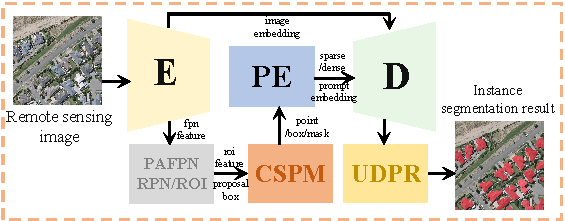
\includegraphics[width=\columnwidth]{总体架构简图.pdf}
\caption{Overall Architecture of PromptMiner-SAM2}
\label{fig:arch}
\vspace{-0.7em}
\end{figure}

Each proposal $b_r$ anchors its multi-level RoIAlign feature $X_r$ and all
prompts in an image-aligned prompt coordinate frame. SAM2 decodes the image embedding with these
proposal-specific prompts, and the resulting upscaled features enter UDPR.
Points encode interior/exterior cues, the box constrains extent, and the dense
prompt supplies a local shape prior.

\subsection{Coarse-Shape Prompt Mining (CSPM)}
For each proposal, the coarse branch maps its RoI feature $X_r$ to a
proposal-local shape logit map
\begin{equation}
C_r=f_{\mathrm{coarse}}(X_r),\qquad C_r\in\mathbb{R}^{1\times64\times64}.
\label{eq:coarse}
\end{equation}
Figure~\ref{fig:cspm} summarizes the conversion of the coarse shape into the
three SAM2 prompt types.
\begin{figure}[t]
\centering
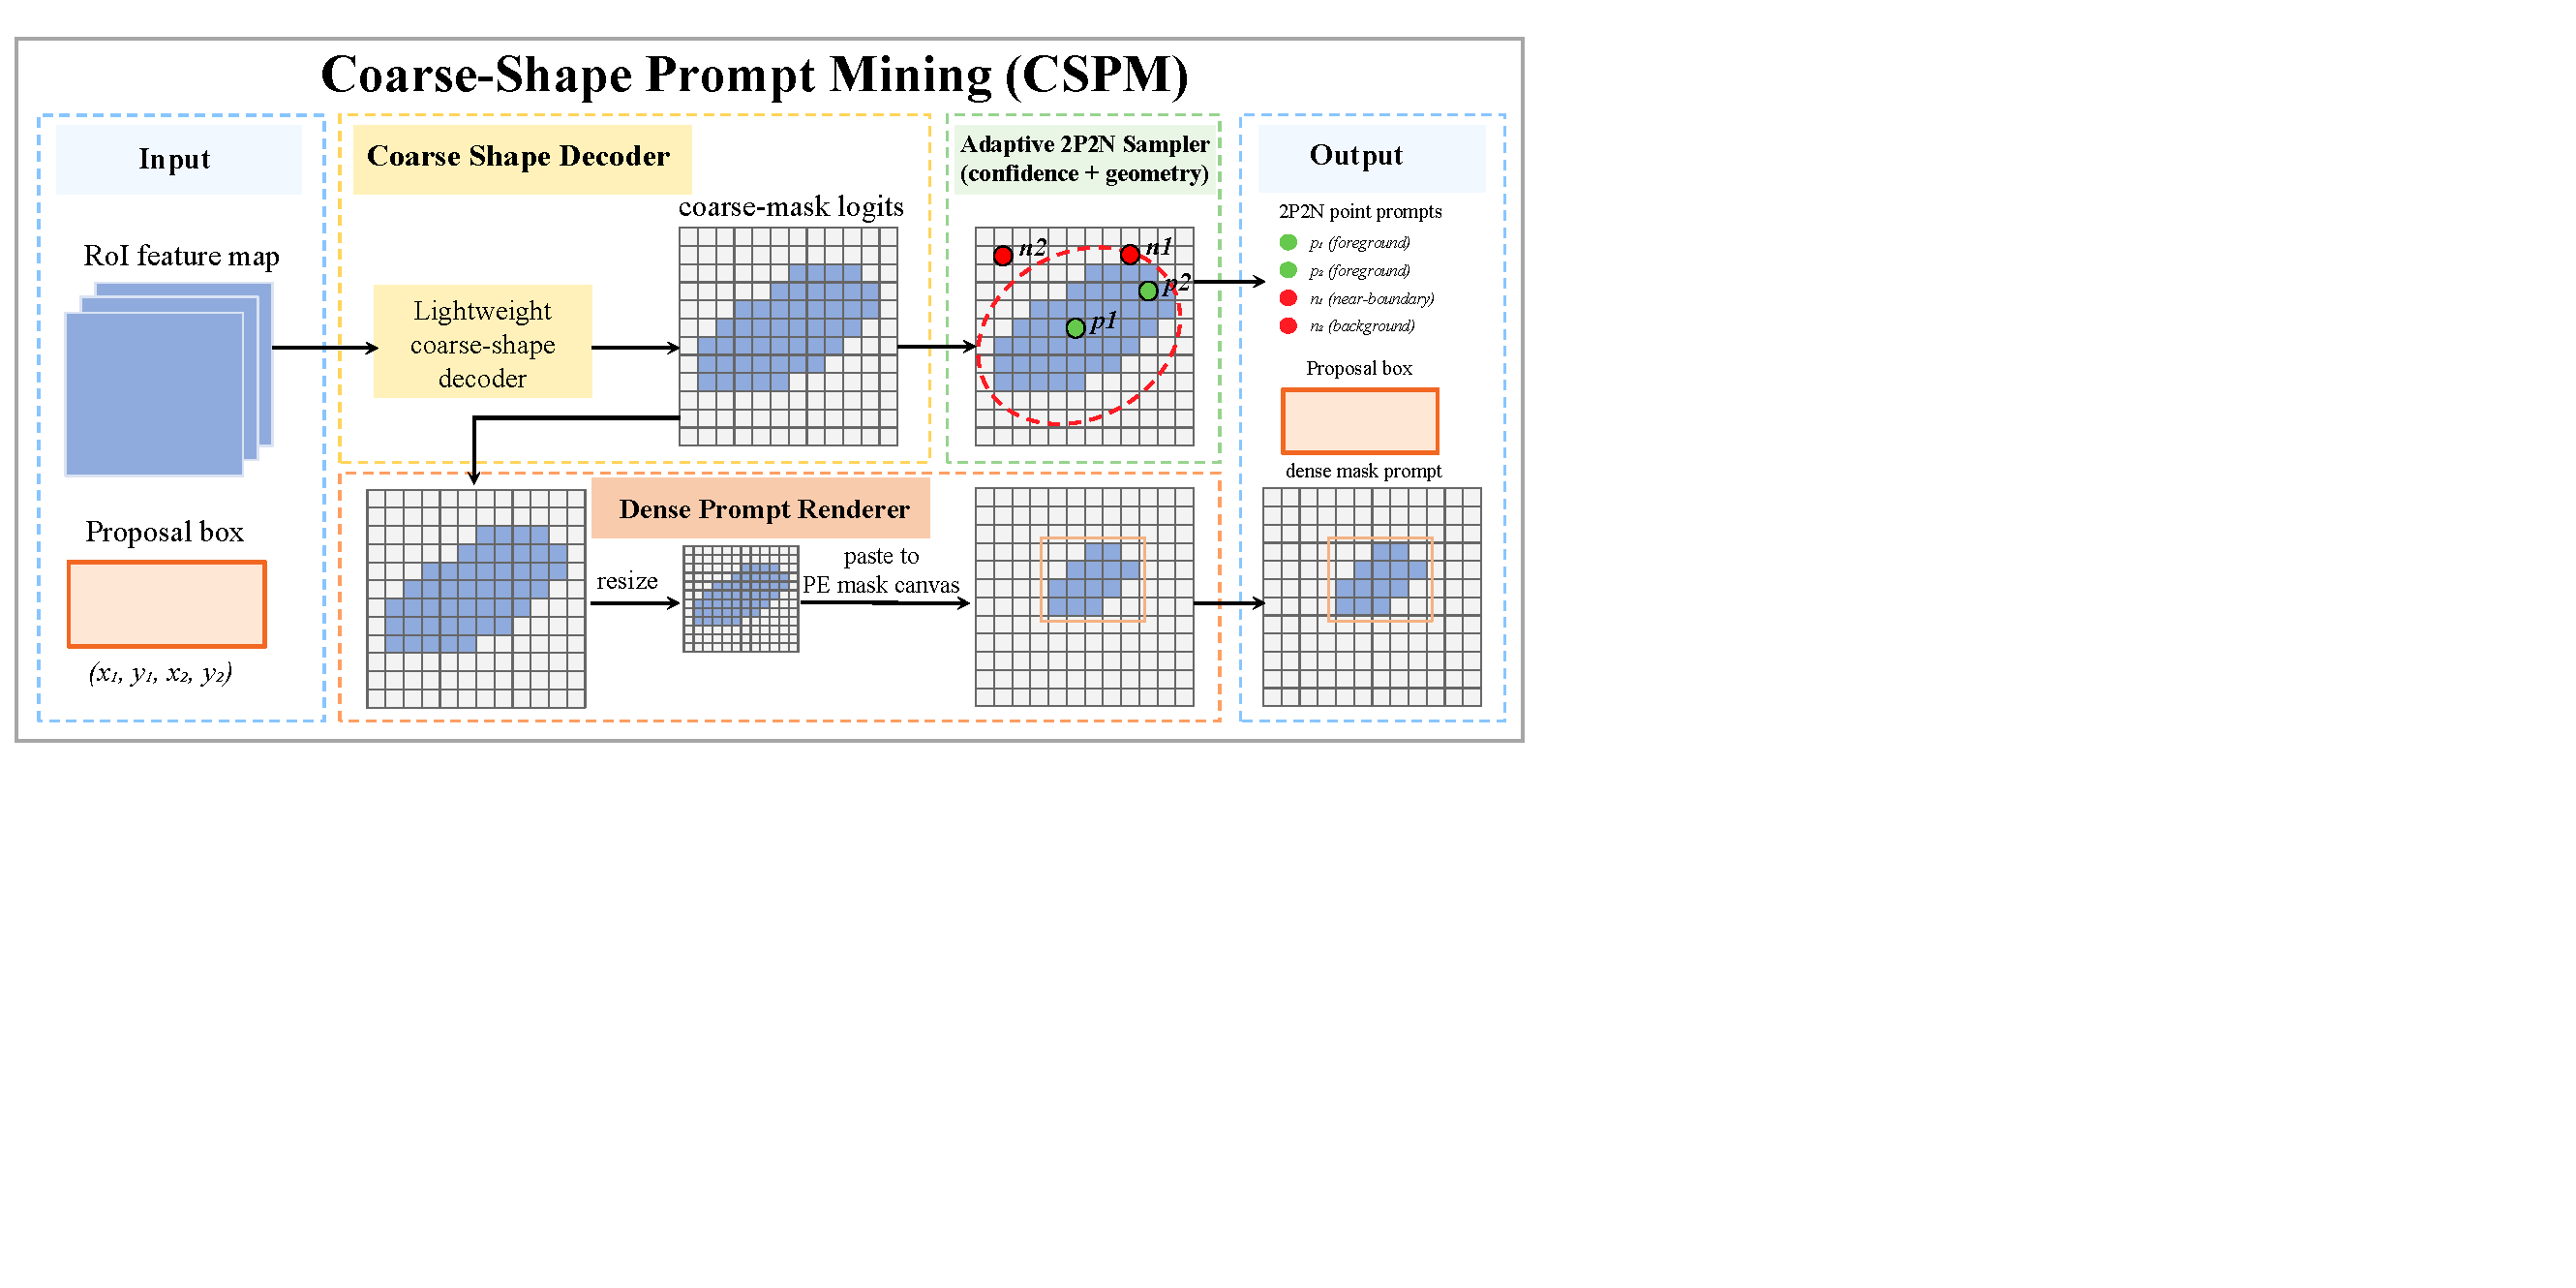
\includegraphics[width=\columnwidth]{CSPM.pdf}
\caption{Coarse-shape prompt mining (CSPM).}
\label{fig:cspm}
\vspace{-0.8em}
\end{figure}
Let $p_r=\sigma(C_r)$. PromptMiner derives a foreground support at probability
$0.5$ from $p_r$, while retaining the signed logits $C_r$ for the dense prompt.
It mines two positive and two negative points (2P2N) from this shared coarse
shape. The first positive point is selected among confident foreground interior
pixels ($p_r\geq0.6$) by its foreground confidence weighted by its normalized
distance to the support boundary; the second follows the same criterion while
remaining spatially separated from the first. The first negative point comes
from the one-pixel outer ring with low foreground probability ($p_r\leq0.3$).
The second is selected from background outside a dilation of the foreground
support and is separated from the first positive and ring-negative points.

This construction assigns distinct geometric roles to the four points. The
positive pair anchors the object interior without repeatedly sampling one local
peak. In contrast, the ring negative is tied to the immediate exterior of the
coarse shape, whereas the second negative represents a less local background
context. The 2P2N set records the coarse shape as sparse signed point prompts
before they are transferred from the RoI frame to the image frame.

The resulting coordinates and positive/negative labels are mapped from the
RoI frame to image coordinates. In parallel, the signed coarse logits are resized
to the support of $b_r$ and pasted onto the mask-input canvas:
\begin{equation}
\mathcal{S}_r=\mathcal{M}(C_r,b_r),\qquad
Q_r=\operatorname{Place}(C_r,b_r),
\label{eq:prompt-mining}
\end{equation}
Here, $\mathcal{M}$ denotes 2P2N selection and coordinate mapping, and
$\operatorname{Place}$ is the resize-and-paste operation. The two corners of
$b_r$ provide the box prompt. SAM2 jointly encodes the point, box, and
dense-mask prompts, then decodes them with the image embedding in one pass:
\begin{equation}
Y_r^0=\mathcal{D}\bigl(\mathcal{E}_I(I),
\widetilde{\mathcal{E}}_P(\mathcal{S}_r,b_r,Q_r)\bigr),
\label{eq:native-decoding}
\end{equation}
where $\mathcal{E}_I$, $\widetilde{\mathcal{E}}_P$, and $\mathcal{D}$ denote
the SAM2 image encoder (including its decoder-side high-resolution features),
complete SAM2 prompt-embedding pathway, and mask decoder, respectively.
The pathway $\widetilde{\mathcal{E}}_P$ includes the SAM2 composition of
the dense-mask embedding. $Q_r$ retains the signed rather than binarized
coarse logits. Thus, the dense prompt preserves the spatial variation of the
proposal-local shape, while the point and box prompts provide discrete
geometric constraints to the same decoder.

\subsection{Uncertainty-Guided Decoder-Tail Refinement (UDPR)}
The same decoding pass also returns an upscaled decoder feature map $U_r$ and
the first output mask token $t_r$, in addition to the decoder logit map $Y_r^0$.
On the raster grid $\mathcal{G}_r$, UDPR visits the $K_r$ locations with
the smallest logit magnitudes, as illustrated in Figure~\ref{fig:udpr}:
\begin{equation}
\begin{aligned}
K_r&=\min(K,|\mathcal{G}_r|),\\
\Omega_r&=\operatorname{BottomK}\bigl(|Y_r^0|,K_r\bigr),\qquad K=64,
\end{aligned}
\label{eq:udpr-selection}
\end{equation}
\begin{figure}[t]
\centering
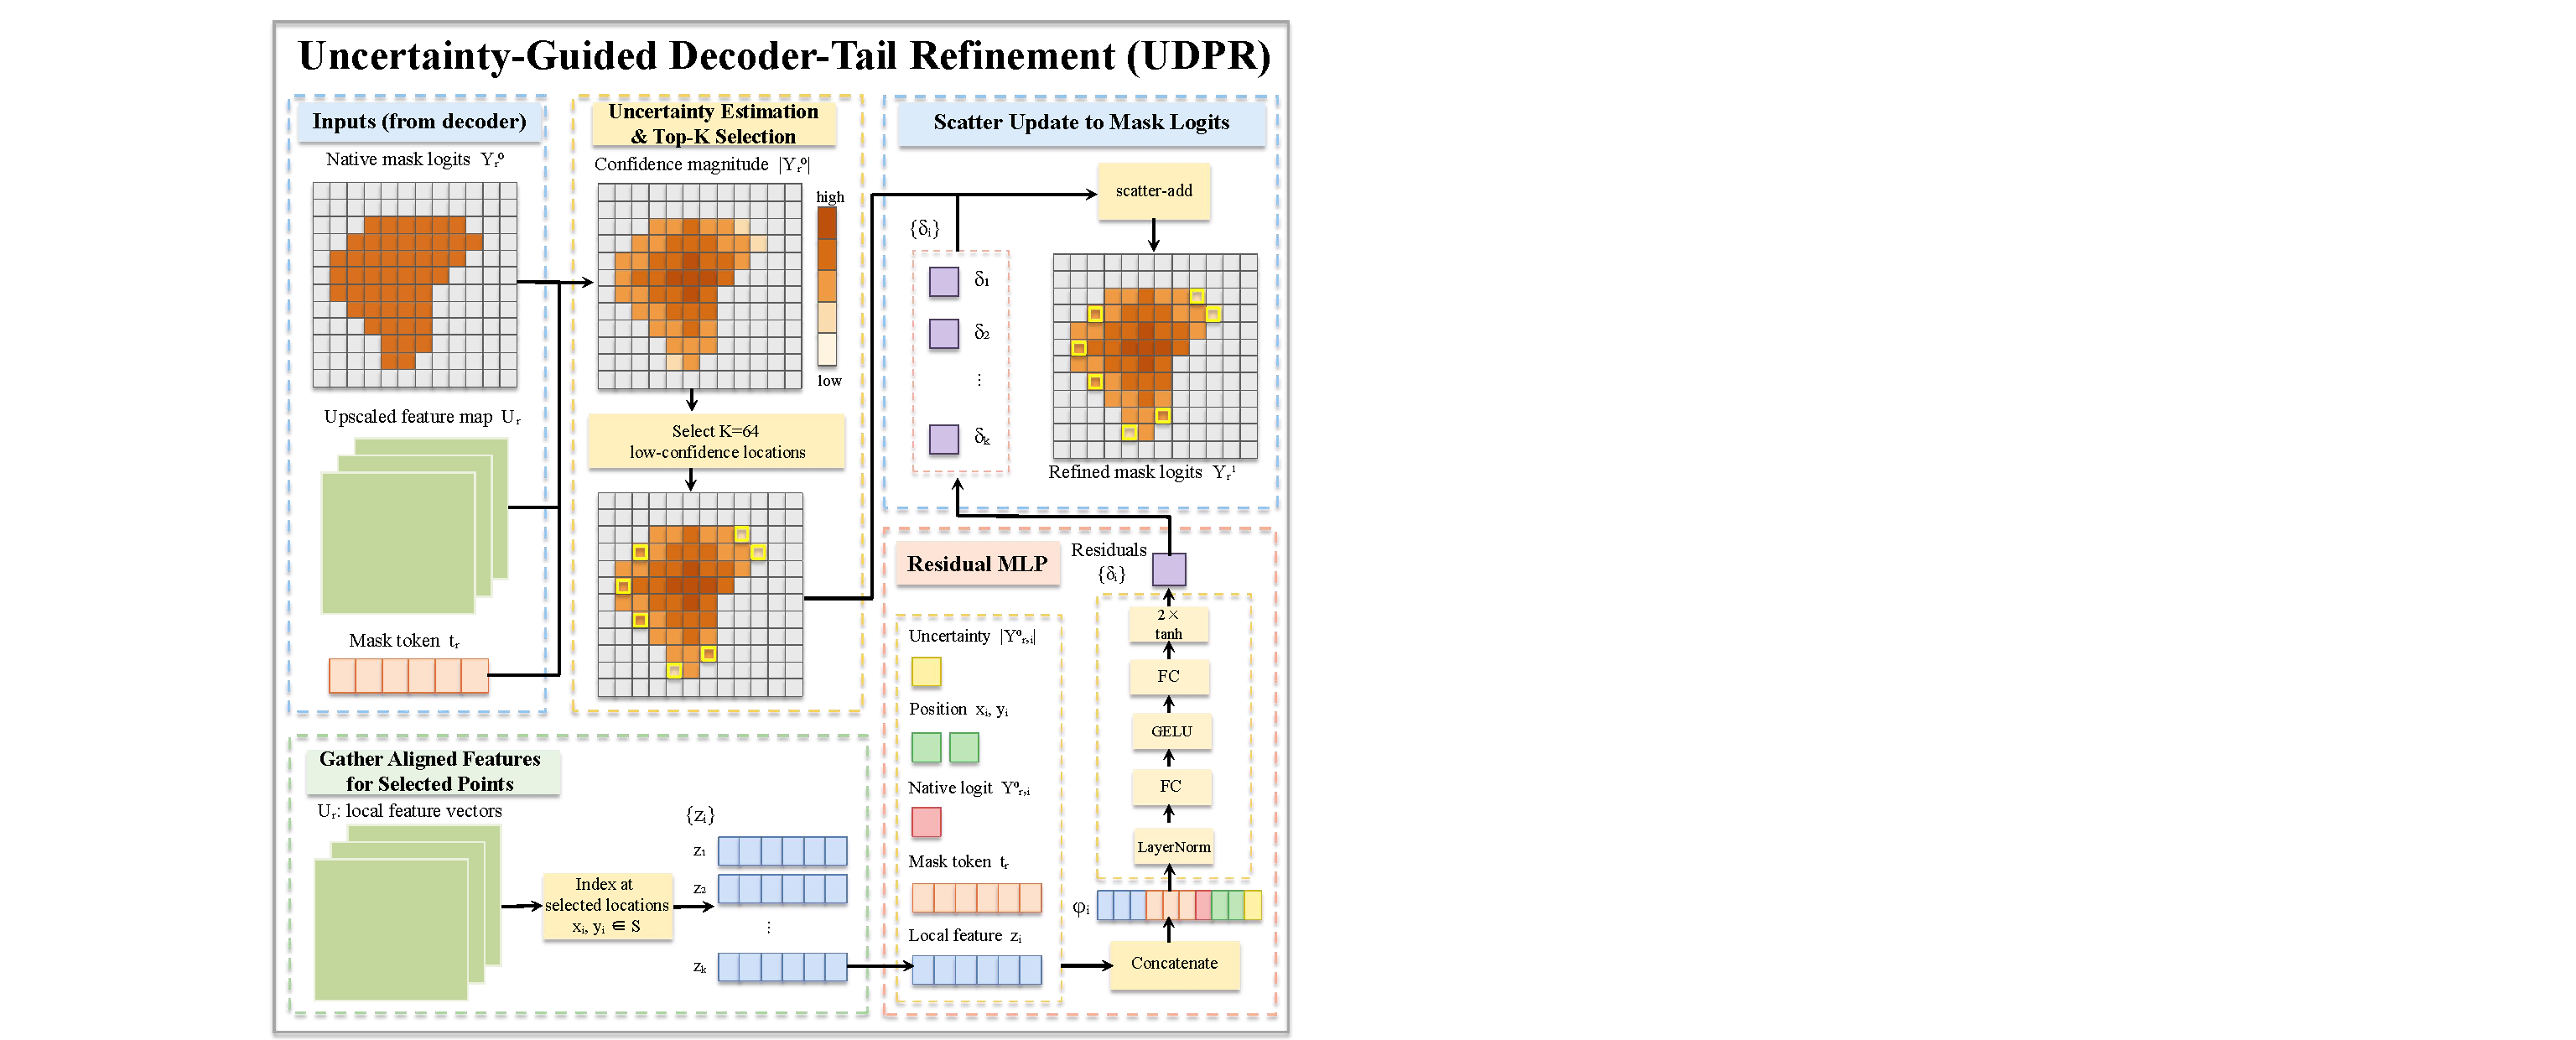
\includegraphics[width=\columnwidth]{UDPR.pdf}
\caption{Uncertainty-guided decoder-tail refinement (UDPR).}
\label{fig:udpr}
\vspace{-0.8em}
\end{figure}
where $\operatorname{BottomK}$ returns the $K_r$ indices in $\mathcal{G}_r$
with the smallest logit magnitudes.
For each $i\in\Omega_r$, the aligned feature $z_i$ is gathered from $U_r$ and
combined with the token, normalized location, local logit, and logit magnitude:
\begin{equation}
\phi_i=[z_i,t_r,Y^0_{r,i},x_i,y_i,|Y^0_{r,i}|].
\label{eq:udpr-input}
\end{equation}
The local feature describes the decoder output near $i$, the mask token
conditions the update on the decoded instance, and the coordinate and logit
terms specify the position and current decision state. A lightweight MLP $g$
then predicts a bounded residual for each selected location:
\begin{equation}
\delta_i=2\tanh g(\phi_i),\qquad i\in\Omega_r,
\label{eq:udpr}
\end{equation}
The refined logit map is formed by scattering these residuals back to their
original positions:
\begin{equation}
Y^1_{r,i}=\begin{cases}
Y^0_{r,i}+\delta_i, & i\in\Omega_r,\\
Y^0_{r,i}, & i\notin\Omega_r.
\end{cases}
\label{eq:udpr-scatter}
\end{equation}
This selective update leaves all nonselected decoder logits unchanged and
uses the outputs of the single prompt-conditioned decoding pass throughout.

\section{EXPERIMENTS}
\subsection{Training Details}
Our implementation uses PyTorch and distributed data parallelism on four NVIDIA RTX 3090 GPUs. 
Each GPU processes one image and gradients are accumulated for two iterations, resulting in an effective global batch size of eight. 
We train with automatic mixed precision and AdamW (initial learning rate $5\times10^{-4}$, weight decay $0.05$, and $\epsilon=10^{-6}$). 
The learning rate is linearly warmed up for the first 100 optimizer steps from $0.1\%$ of its initial value, followed by cosine annealing to $0.1\%$ of that value. 
Training uses cross-entropy, Smooth L1, binary cross-entropy, and Dice losses.

\subsection{Evaluation Protocol and Comparisons}
We evaluate on the WHU dataset~\cite{whu}, a single-class building benchmark with a
2,943/627/2,220 train/validation/test split, and NWPU VHR-10~\cite{nwpu}, a
ten-class benchmark. Since NWPU VHR-10 originally provides detection annotations
only, we use the publicly released instance masks of Su \textit{et al.}~\cite{nwpu_instance}
and its 520/130 train/evaluation split. We use COCO-style bbox and mask AP, AP$_{50}$, and
AP$_{75}$. Table~\ref{tab:comparison} reports
the comparative results under this
evaluation protocol. To assess the proposed method, we compare it with
11 representative instance-segmentation methods. These
methods fall into two broad groups: CNN-based methods, including two-stage,
one-stage, and cascade designs; and methods that exploit global sequence
modeling, including transformer-style mask prediction and foundation-model
prompting. This comparison includes conventional instance-segmentation
pipelines and methods with global sequence modeling.

\begin{figure*}[t]
\centering
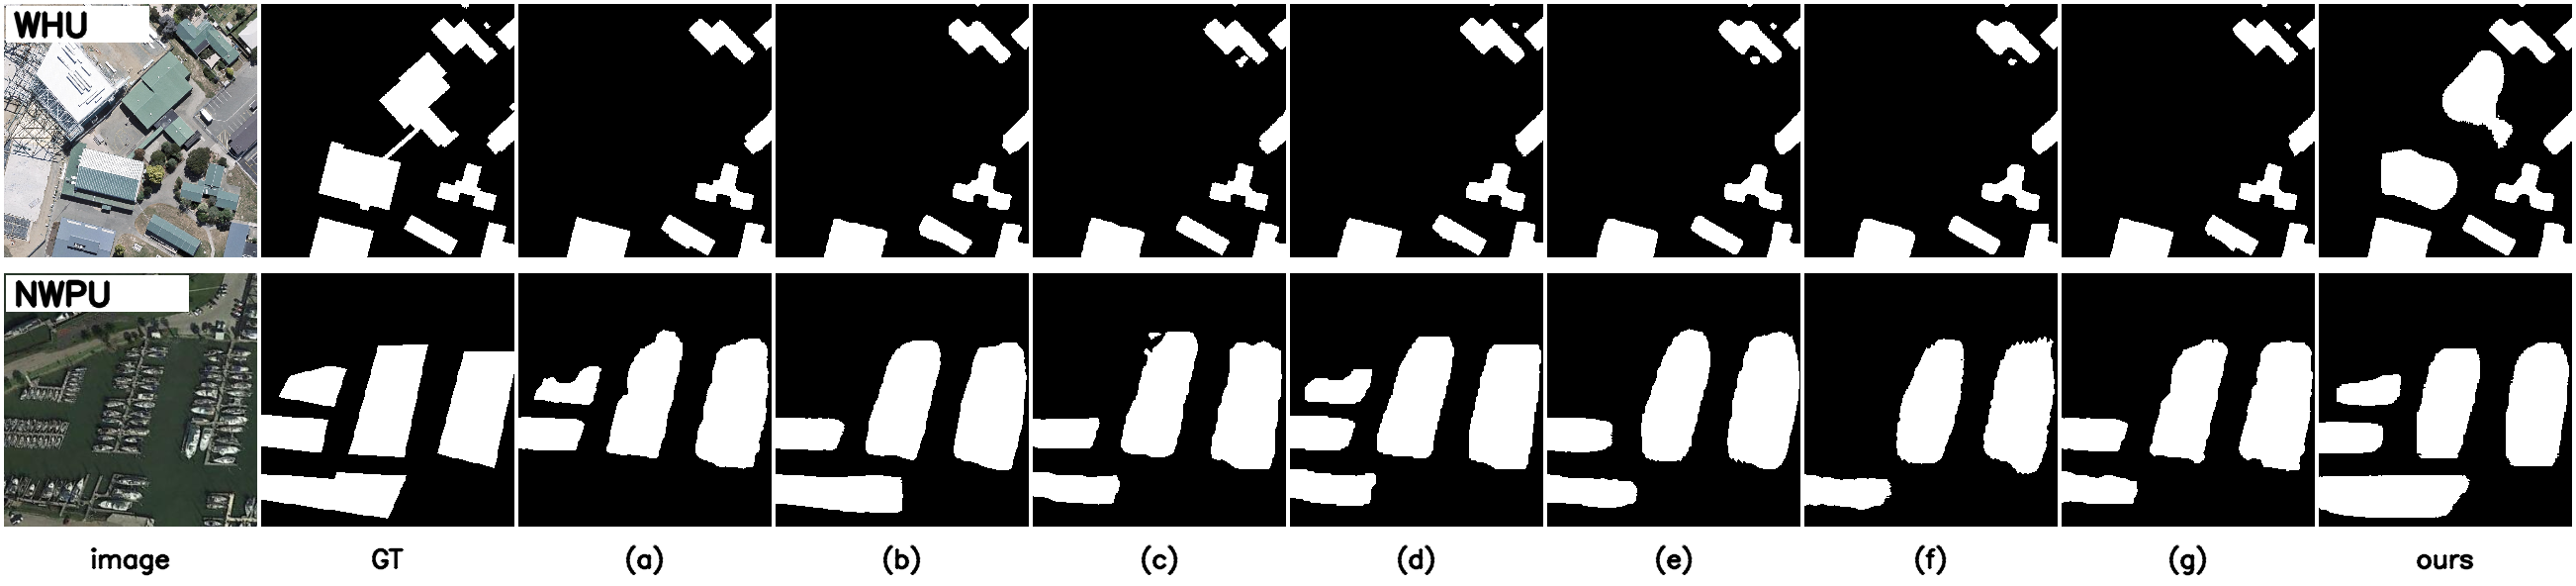
\includegraphics[width=\textwidth]{viz_grid_row_combined.png}
\caption{Qualitative comparison on the WHU and NWPU VHR-10 datasets. From left to right, the columns show the input image, ground truth, predictions of (a) MaskDINO, (b) RSPrompter, (c) CondInst, (d) YOLO11, (e) HTC, (f) Mask R-CNN, (g) M2F, and PromptMiner-SAM2 (ours).}
\label{fig:qualitative}
\end{figure*}

\begin{table*}[t]
\caption{Comparative analysis on the WHU and NWPU VHR-10 datasets. Each entry reports AP / AP$_{50}$ / AP$_{75}$ (\%) for boxes or masks.}
\label{tab:comparison}
\centering
\scriptsize
\begingroup
\setlength{\tabcolsep}{7pt}
\renewcommand{\arraystretch}{1.08}
\resizebox{\textwidth}{!}{%
\begin{tabular}{llcccc}
\toprule
& & \multicolumn{2}{c}{WHU} & \multicolumn{2}{c}{NWPU VHR-10} \\
\cmidrule(lr){3-4}\cmidrule(lr){5-6}
& & Bbox (\%) & Mask (\%) & Bbox (\%) & Mask (\%) \\
\cmidrule(lr){3-3}\cmidrule(lr){4-4}\cmidrule(lr){5-5}\cmidrule(lr){6-6}
Type & Method & \metricheader & \metricheader & \metricheader & \metricheader \\
\midrule
\multirow{6}{*}{\textit{CNN-based}} & Mask R-CNN~\cite{maskrcnn} & \metrictriplet{70.9}{89.9}{80.9} & \metrictriplet{68.2}{90.0}{80.0} & \metrictriplet{50.1}{82.1}{57.7} & \metrictriplet{49.1}{81.7}{50.5} \\
& MS R-CNN~\cite{msrcnn} & \metrictriplet{68.8}{89.4}{80.0} & \metrictriplet{67.7}{89.6}{79.5} & \metrictriplet{51.5}{85.2}{59.2} & \metrictriplet{52.7}{82.6}{56.8} \\
& HTC~\cite{htc} & \metrictriplet{72.7}{90.6}{82.5} & \metrictriplet{69.2}{90.7}{81.6} & \metrictriplet{58.9}{86.9}{67.7} & \metrictriplet{51.3}{84.6}{53.3} \\
& CondInst~\cite{condinst} & \metrictriplet{74.2}{90.0}{82.4} & \metrictriplet{69.7}{90.2}{80.9} & \metrictriplet{65.0}{90.1}{79.6} & \metrictriplet{62.8}{90.7}{68.1} \\
& RTMDet-Ins-S~\cite{rtmdet} & \metrictriplet{64.2}{85.6}{75.3} & \metrictriplet{59.8}{85.8}{71.2} & \metrictriplet{59.6}{91.5}{70.6} & \metrictriplet{46.3}{79.2}{47.2} \\
& YOLO11s-seg~\cite{yolo11} & \metrictriplet{\textbf{76.7}}{91.2}{\textbf{85.4}} & \metrictriplet{66.8}{91.3}{79.1} & \metrictriplet{71.0}{\textbf{94.4}}{79.5} & \metrictriplet{63.9}{93.9}{67.3} \\
\midrule
\multirow{5}{*}{\shortstack{\textit{Global sequence}\\\textit{modeling}}} & Mask2Former~\cite{mask2former} & \metrictriplet{61.4}{82.7}{70.7} & \metrictriplet{64.5}{84.1}{75.6} & \metrictriplet{60.3}{77.9}{66.8} & \metrictriplet{61.5}{84.9}{67.8} \\
& MaskDINO~\cite{maskdino} & \metrictriplet{73.3}{90.8}{82.7} & \metrictriplet{73.3}{90.3}{82.5} & \metrictriplet{65.7}{88.9}{74.2} & \metrictriplet{65.8}{89.6}{71.5} \\
& RS4D-box~\cite{rs4d} & \metrictriplet{64.5}{87.6}{74.7} & \metrictriplet{64.1}{87.8}{75.2} & \metrictriplet{57.0}{82.5}{65.4} & \metrictriplet{54.3}{80.1}{57.6} \\
& RSIISN~\cite{rsiisn} & \metrictriplet{74.1}{90.0}{84.4} & \metrictriplet{72.1}{90.1}{83.9} & \metrictriplet{58.1}{89.3}{66.8} & \metrictriplet{62.9}{89.7}{67.1} \\
& RSPrompter~\cite{rsprompter} & \metrictriplet{72.5}{91.0}{81.7} & \metrictriplet{72.5}{\textbf{92.0}}{82.9} & \metrictriplet{70.3}{93.6}{81.0} & \metrictriplet{66.1}{92.7}{70.6} \\
\midrule
Ours & PromptMiner-SAM2 & \metrictriplet{76.4}{\textbf{91.5}}{\textbf{85.4}} & \metrictriplet{\textbf{73.4}}{91.4}{\textbf{85.5}} & \metrictriplet{\textbf{72.8}}{93.9}{\textbf{84.0}} & \metrictriplet{\textbf{67.8}}{\textbf{95.4}}{\textbf{74.0}} \\
\bottomrule
\end{tabular}
}
\endgroup
\end{table*}

Quantitatively, PromptMiner-SAM2 obtains the highest mask AP on both
benchmarks. On the WHU dataset, it reaches 73.4\% mask AP and 85.5\% mask
AP$_{75}$, exceeding the strongest competing results by 0.1 and 1.6 points,
respectively. Its bbox AP of 76.4\% is also competitive, only 0.3 points
below the best result. On NWPU VHR-10, our method achieves the best bbox AP
(72.8\%), bbox AP$_{75}$ (84.0\%), mask AP (67.8\%), mask AP$_{50}$
(95.4\%), and mask AP$_{75}$ (74.0\%).

Figure~\ref{fig:qualitative} provides qualitative comparisons on the two
benchmarks. In densely built or visually ambiguous areas, where shadows, weak
roof contrast, and narrow inter-building gaps complicate instance delineation,
PromptMiner-SAM2 recovers more complete building footprints and produces
cleaner separations between adjoining instances. These visual differences are
consistent with its stronger high-IoU mask accuracy in Table~\ref{tab:comparison}.

\FloatBarrier
\subsection{Ablation Study}
Table~\ref{tab:ablation} reports the effect of prompt composition and
decoder-tail refinement on NWPU VHR-10. All variants use the same data split,
initialization, training schedule, and checkpoint-selection rule. Starting
from point prompts ($P$), adding the proposal box ($P{+}B$) raises mask AP
from 63.0\% to 65.3\% and mask AP$_{75}$ from 67.4\% to 71.7\%, respectively.
This 2.3-point mask-AP gain, obtained without a corresponding bbox gain,
shows that the box primarily resolves instance extent for mask decoding rather
than improving proposal localization. Adding the dense-mask prompt
($P{+}B{+}M$) further raises mask AP to 65.9\% and bbox AP to 72.1\%. Thus,
the dense prompt transfers coarse shape information beyond the discrete point
and box prompts, although its isolated improvement at AP$_{75}$ is modest.

Adding UDPR to $P{+}B{+}M$ raises mask AP/AP$_{75}$ from 65.9/71.5\% to
67.8/74.0\%, and increases bbox AP$_{75}$ by 2.9 points. Across the complete
path, the gains over $P$ reach 4.8 mask-AP and 6.6 AP$_{75}$ points, showing
that CSPM improves shape conditioning while UDPR strengthens high-IoU masks.

\begin{table}[H]
\caption{Prompt-path ablation on NWPU VHR-10. $P$, $B$, and $M$ denote point, box, and dense-mask prompts.}
\label{tab:ablation}
\centering
\scriptsize
\resizebox{\columnwidth}{!}{%
\begin{tabular}{lcccccc}
\toprule
& \multicolumn{3}{c}{Bbox (\%)} & \multicolumn{3}{c}{Mask (\%)} \\
\cmidrule(lr){2-4}\cmidrule(lr){5-7}
Variant & AP & AP$_{50}$ & AP$_{75}$ & AP & AP$_{50}$ & AP$_{75}$ \\
\midrule
$P$ & 71.8 & 93.6 & 81.9 & 63.0 & 92.6 & 67.4 \\
$P{+}B$ & 71.7 & 93.5 & 81.7 & 65.3 & 93.5 & 71.7 \\
$P{+}B{+}M$ & 72.1 & \textbf{94.4} & 81.1 & 65.9 & 93.5 & 71.5 \\
$P{+}B{+}M$ + UDPR & \textbf{72.8} & 93.9 & \textbf{84.0} & \textbf{67.8} & \textbf{95.4} & \textbf{74.0} \\
\bottomrule
\end{tabular}
}
\end{table}

\section{CONCLUSION}
PromptMiner-SAM2 couples two-stage proposals with SAM2 through coarse-shape
prompts and UDPR. CSPM transforms each proposal-local shape into aligned point,
box, and dense-mask prompts in SAM2's native interface, reducing ambiguity
between adjacent buildings. UDPR selectively updates low-confidence decoder
logits to improve boundary-sensitive masks while preserving confident regions.
The resulting design achieves strong performance on both benchmarks.

\clearpage
\bibliographystyle{IEEEbib}
\begin{thebibliography}{99}
\bibitem{sam} A.~Kirillov \textit{et al.}, ``Segment Anything,'' in \textit{Proc. ICCV}, 2023, pp.~4015--4026.
\bibitem{sam2} N.~Ravi \textit{et al.}, ``SAM 2: Segment Anything in Images and Videos,'' in \textit{Proc. ICLR}, 2025.
\bibitem{samrs} D.~Wang \textit{et al.}, ``SAMRS: Scaling-up remote sensing segmentation dataset with Segment Anything Model,'' in \textit{Adv. Neural Inf. Process. Syst.}, vol.~36, 2023.
\bibitem{rsprompter} K.~Chen \textit{et al.}, ``RSPrompter: Learning to prompt for remote sensing instance segmentation based on visual foundation model,'' \textit{IEEE Trans. Geosci. Remote Sens.}, vol.~62, 2024.
\bibitem{aopsam} Y.~Chen, M.~Son, C.~Hua, and J.-Y.~Kim, ``AoP-SAM: Automation of prompts for efficient segmentation,'' in \textit{Proc. AAAI Conf. Artif. Intell.}, vol.~39, no.~2, pp.~2284--2292, 2025.
\bibitem{pasam} Z.~Xie, B.~Guan, W.~Jiang, M.~Yi, Y.~Ding, H.~Lu, and L.~Zhang, ``PA-SAM: Prompt adapter SAM for high-quality image segmentation,'' in \textit{Proc. IEEE Int. Conf. Multimedia Expo (ICME)}, 2024, pp.~1--6.
\bibitem{samrefiner} Y.~Lin, H.~Li, W.~Shao, Z.~Yang, J.~Zhao, X.~He, P.~Luo, and K.~Zhang, ``SAMRefiner: Taming Segment Anything Model for Universal Mask Refinement,'' in \textit{Proc. Int. Conf. Learn. Represent. (ICLR)}, 2025.
\bibitem{maskrcnn} K.~He, G.~Gkioxari, P.~Doll\'ar, and R.~Girshick, ``Mask R-CNN,'' in \textit{Proc. IEEE Int. Conf. Comput. Vis. (ICCV)}, 2017, pp.~2961--2969.
\bibitem{msrcnn} Z.~Huang, L.~Huang, Y.~Gong, C.~Huang, and X.~Wang, ``Mask Scoring R-CNN,'' in \textit{Proc. IEEE/CVF Conf. Comput. Vis. Pattern Recognit. (CVPR)}, 2019, pp.~6409--6418.
\bibitem{htc} K.~Chen \textit{et al.}, ``Hybrid task cascade for instance segmentation,'' in \textit{Proc. IEEE/CVF Conf. Comput. Vis. Pattern Recognit. (CVPR)}, 2019, pp.~4974--4983.
\bibitem{condinst} Z.~Tian, C.~Shen, and H.~Chen, ``Conditional convolutions for instance segmentation,'' in \textit{Proc. Eur. Conf. Comput. Vis. (ECCV)}, 2020, pp.~282--298.
\bibitem{solov2} X.~Wang, R.~Zhang, T.~Kong, L.~Li, and C.~Shen, ``SOLOv2: Dynamic and fast instance segmentation,'' in \textit{Adv. Neural Inf. Process. Syst.}, vol.~33, 2020, pp.~17721--17732.
\bibitem{mask2former} B.~Cheng, I.~Misra, A.~G.~Schwing, A.~Kirillov, and R.~Girdhar, ``Masked-attention mask transformer for universal image segmentation,'' in \textit{Proc. IEEE/CVF Conf. Comput. Vis. Pattern Recognit. (CVPR)}, 2022, pp.~1290--1299.
\bibitem{rtmdet} C.~Lyu \textit{et al.}, ``RTMDet: An empirical study of designing real-time object detectors,'' \textit{arXiv preprint arXiv:2212.07784}, 2022.
\bibitem{yolo11} G.~Jocher and J.~Qiu, ``Ultralytics YOLO11,'' software, ver.~11.0.0, 2024. [Online]. Available: \url{https://github.com/ultralytics/ultralytics}
\bibitem{maskdino} F.~Li \textit{et al.}, ``Mask DINO: Towards a unified transformer-based framework for object detection and segmentation,'' in \textit{Proc. IEEE/CVF Conf. Comput. Vis. Pattern Recognit. (CVPR)}, 2023, pp.~3041--3050.
\bibitem{rs4d} Q.~Yang, K.~Chen, J.~Xu, Z.~Shi, and Z.~Zou, ``Efficient remote sensing instance segmentation with linear-time state space distilled visual foundation models,'' \textit{arXiv preprint arXiv:2606.25324}, 2026.
\bibitem{rsiisn} W.~Ye, W.~Zhang, W.~Lei, W.~Zhang, X.~Chen, and Y.~Wang, ``Remote sensing image instance segmentation network with transformer and multi-scale feature representation,'' \textit{Expert Syst. Appl.}, vol.~234, Art.~no.~121007, 2023.
\bibitem{p2pformer} T.~Zhang, S.~Wei, Y.~Zhou, M.~Luo, W.~Yu, and S.~Ji, ``P2PFormer: A primitive-to-polygon method for regular building contour extraction from remote sensing images,'' \textit{IEEE Trans. Geosci. Remote Sens.}, vol.~62, Art.~no.~4414012, 2024.
\bibitem{whu} X.~Xia, Z.~Sun, S.~Ji, P.~Dong, and W.~Li, ``WHU Building Dataset,'' 2018. [Online]. Available: \url{https://study.rsgis.whu.edu.cn/pages/download/}
\bibitem{nwpu} G.~Cheng, J.~Han, P.~Zhou, and L.~Guo, ``Multi-class geospatial object detection and geographic image classification based on collection of part detectors,'' \textit{ISPRS J. Photogramm. Remote Sens.}, vol.~98, pp.~119--132, 2014.
\bibitem{nwpu_instance} H.~Su, S.~Wei, M.~Yan, C.~Wang, J.~Shi, and X.~Zhang, ``Object detection and instance segmentation in remote sensing imagery based on precise Mask R-CNN,'' in \textit{Proc. IEEE Int. Geosci. Remote Sens. Symp. (IGARSS)}, 2019, pp.~1454--1457.
\end{thebibliography}
\end{document}
